\documentclass{beamer}
\usepackage {beamerthemeWarsaw}
\usepackage{graphicx}
\DeclareGraphicsExtensions{.pdf,.png,.jpg}
\setbeamerfont{structure}{family=\rmfamily,shape=\itshape} 
\usepackage{times}
\usepackage[orientation=landscape,size=custom,width=16,height=9,scale=0.5,debug]{beamerposter}
\usepackage{graphicx}
\usepackage{caption} 
\begin{document}



\title{Quantitative Analysis of Acid Base Disorder}   
\author{Mohamad Atef Radwan} 

\date{\today} 
{\usebackgroundtemplate{
\includegraphics[width=\paperwidth,
height=\paperheight]{fract1}
}
\frame{

\titlepage
\centerline{Resident of Anesthesia and  SICU}} }
\frame{
\frametitle{Objectives}

\begin{figure}[htb]
\begin{center}
\leavevmode
\includegraphics[width=.3\textwidth]{imgs/objective}
\end{center}

\end{figure}

\begin{itemize}
\item Idea about history of interpretation (Boston And Copenhagen)
\item Understanding Mathematical Concept of Stewart approach
\item Quantitative Interpretation of Acid Base disturbances
\item Clinical Application of Stewart approach 
\end{itemize}
}
\frame{
\frametitle{Story started from HH}
\begin{itemize}
	\item Aim: Maintain pH of solution
	\item Method : You should have \textit{Buffer} 
\end{itemize}


\begin{block}{Method}
Classical buffer contains solution of weak acid and conjugate base. Small amounts of acids or bases added are absorbed by buffer and the pH changes only slightly...
\end{block}



}
\frame{
\frametitle{Bicarbonate Buffer System}

\Large \begin{equation*}[H^{+}]=K_{a} \tfrac{HA}{A^{-}}\end{equation*}
\begin{alertblock}{HH Equation}
\Large \begin{equation*}pH = pK_{a}+log_{10} [\tfrac{HCO3^{-}}{0.03*PaCO_{2}}]\end{equation*}
\end{alertblock}
}
\frame{
\frametitle{So...}
\begin{block}{Simply}
\large \begin{equation*}pH \propto [\tfrac{HCO3^{-}}{PaCO_{2}}]\end{equation*}
For disturbing  H$^{+}$ Concentration:
\begin{itemize}
\item HCO3$^{-}$ Increase or Decrease
\item PaCO$_{2}$ Increase Or Decrease 
\end{itemize}
\end{block}
\textbf{Controllers :\textit{Lungs, Kidney, Liver}}
}
\frame{
\frametitle{Compensation }
\Large \begin{equation*}pH \propto [\tfrac{HCO3^{-}\uparrow \downarrow}{PaCO_{2}\uparrow \downarrow }]\end{equation*}
\begin{itemize}
\large\item CO$_{2}$ = Respiratory = Lung
\large\item HCO3$^{-}$ = Metabolic = Kidney
\end{itemize}
}
\frame{
\frametitle{Boston...}
\begin{columns}[c] % the "c" option specifies center vertical alignment
\column{.5\textwidth} % column designated by a command
\begin{block}{6 types of Disorder}

\begin{itemize}
\item Acute Respiratory Acidosis 
\item Chronic Respiratory Acidosis
\item Acute Respiratory Alkalosis
\item Chronic Respiratory Alkalosis
\item Metabolic Acidosis
\item Metabolic Alkalosis
\end{itemize}
\end{block}
\column{.5\textwidth}
	\begin{figure}[htb]

\leavevmode
\includegraphics[width=0.8\textwidth]{imgs/six}
\end{figure}
\end{columns}

}
\frame{
\frametitle{Winter Rules}
\begin{itemize}

\item The rules describe the normal physiological reactions of the human body to one isolated acid-base Disorder\\
\item The clinical question the rules are designed to answer in this situation is, whether the patient's respiratory compensation is within the range to be expected or whether there is an additional component of respiratory disturbance\\
\item Example :: DKA with Respiratory Compensation
\end{itemize}
}
\frame{
\frametitle{Winter rules }
\begin{figure}[htb]
\begin{center}
\leavevmode
\includegraphics[width=1\textwidth]{imgs/winter_mod}
\end{center}

\end{figure}

}
\frame{
\frametitle{ \small \textit{Assessing acid-base disorders, Kidney International ..copied from acidbase.org}}
\begin{center}
\begin{figure}[htb]
\leavevmode
\includegraphics[width=0.8\textwidth]{imgs/winter.png}
\end{figure}
\end{center}

}
\frame{
\frametitle{Indepth:}
\begin{itemize}
\item \textbf{In Metabolic Acidosis}\\
\textit {\textcolor{red}{Anion Gap should be Checked :: High Or Normal ::}}
\item \textbf{In Metabolic Alkalosis}\\ 
\textit{\textcolor{red}{Type should Be known :: Cl Responsive or Resistant ::}}
\end{itemize}
}


\frame{
\frametitle{Henderson and Van Slayk}
\begin{columns}[c] % the "c" option specifies center vertical alignment
\column{.5\textwidth} % column designated by a command

\begin{figure}[htb]
\leavevmode
\includegraphics[width=.5\textwidth]{imgs/f2}
\end{figure}
\column{.5\textwidth}
\begin{figure}[htb]
\leavevmode
\includegraphics[width=1\textwidth]{imgs/van.png}
\end{figure}
\end{columns}
}

\frame{
\frametitle{Siggaard Andersen..The Complete Picture}
\begin{columns}[c]
\column{.3\textwidth} 
\begin{figure}[htb]
\leavevmode
\includegraphics[width=0.8\textwidth]{imgs/a2.png}

\end{figure}

\column{.7\textwidth}
\begin{exampleblock}{}
 1960, Ole Seggard Anderson  25 year old, rotating intern, helped to produce an alignment nomogram relating PCO2 and pH to base Excess
\end{exampleblock}
\end{columns}
}

\frame{
\frametitle{More Buffers..}
\begin{figure}[htb]
\begin{center}
\leavevmode
\includegraphics[width=.55\textwidth]{imgs/singer}
\end{center}

\end{figure}
\begin{exampleblock}{}
\textit{Singer and Hasting} proposed \textbf{buffer base} as  sum of all blood buffers (anions) including \textit{bicarbonate, proteins, and hemoglobin} in one liter of blood
\end{exampleblock}
}

\frame{
\frametitle{Seggard Anderson nomogram}

\begin{columns}[c]
\column{.4\textwidth} 
\begin{figure}[htb]
\leavevmode
\includegraphics[width=1\textwidth]{imgs/san.png}
\end{figure}

\column{.5\textwidth}
\small
\begin{itemize}
\item \textcolor{red}{Point A} : measured pH at high PaCO$_{2}$ 
\item \textcolor{red}{Point B} : measured pH at low PaCO$_{2}$ 

\item \textcolor{red}{Point C} : the BE "Base Exceess"
\item \textcolor{red}{Point D} : the Buffer Base
\end{itemize}
\end{columns}
}

\frame{
\frametitle{So we Can Define }
\begin{block}{Base Excess:}
{The\textbf{ miliequivalents of strong acid or bases} that is needed to titrate one liters (in vitro) of blood or plasma that has been equlibrated to pCO2 = 40 mmhg and to physiological pH of 7.4,at temperature 37 c and full O2 saturation}
\end{block}
\begin{block}{Buffer Base:}
{Is the sum of all buffering agents in the blood including \textbf{bicarbonate, proteins, and hemoglobin} in one liter of blood }
\end{block}
}
\frame{
\frametitle{BE calculation And SBE}

\begin {block}{Van Slayk equation}
BE =   (HCO3     - 24.4  +  [2.3 * Hb + 7.7]  *  [pH -  7.4]) *   (1-  0.023*   Hb)
\end{block}
\begin{figure}[htb]
\begin{center}
\leavevmode
\includegraphics[width=.25\textwidth]{imgs/qs_mod}
\end{center}

\end{figure}


}
\frame{
\frametitle{BE calculation And SBE}
\begin {block}{Van Slayk equation}
BE =   (HCO3$^{-}$     - 24.4  +  [2.3 \times Hb + 7.7]  \times  [pH -  7.4]) \times   (1-  0.023 \times  Hb)
\end{block}
\begin {block}{Standard Base Excess}
SBE  =    0.9287  \times   (HCO3$^{-}$   -   24.4 +14.83  \times  [pH  -  7.4])
\end{block}
}
\frame{
\frametitle{BE Computing Method}
\textbf{Alan W. Grogono}, created java applet for interpretation of acid base disorder using  pH, PCO2 and SBE
\begin{columns}[c]
\column{.5\textwidth} 
\begin{figure}[htb]
\begin{center}
\leavevmode
\includegraphics[width=1\textwidth]{imgs/gor_mod}
\end{center}

\end{figure}

\column{.5\textwidth}
Typical Zones:
\small 
\begin{itemize}
\item Acute Respiratory Acidosis (7 and 8)
\item Chronic Respiratory Acidosis (5)
\item Metabolic Alkalosis (3)
\item Acute Respiratory Alkalosis (18 and 19)
\item Chronic Respiratory Alkalosis (16)
\item Metabolic Acidosis (14)
\end{itemize}
\end{columns}



}
\frame{
\frametitle{Clinical Example}
\begin{center} \Large\textcolor{red}{Running Java Application using AppViewer} \end{center}
}

\frame{
\frametitle{Stewart Approach...\tiny Elephant Idea from acidbase.org}

\begin{center}

\includegraphics[width=0.65\textwidth]{imgs/ele}
\end{center}

}

\frame{
\frametitle{Stewart Approach.. Simply}
\begin{columns}[c]
\column{.5\textwidth} 
\begin{center}What is the role of bicarbonate (HCO3$^{-}$) \\in \\acid-base balance? \\\end{center}
\begin{center}\textit{The answer is simply:}\\\end{center}
\begin{center}\textcolor{red}{None!}\end{center}
\begin{flushright}Peter Stewart (1921-1993)\end{flushright}
\column{.5\textwidth}
\begin{center}\includegraphics[width=0.65\textwidth]{imgs/st_mod}\end{center}

\end{columns}

}
\frame{
\frametitle{Do we need other approach }
Ok ...look to the following Case -Fencle Case 18-, what is your interpretation...

\begin{figure}[htb]
\begin{center}
\leavevmode
\includegraphics[width=.3\textwidth]{imgs/fen}
\end{center}

\end{figure}

\begin{block}{}Chronic obstructive pulmonary disease [COPD], bronchopneumonia, congestive heart failure)
\end{block}
}
\frame{
\frametitle{You may think that the solution my be }
\center\Large Post-Hypercarbic Metabolic Alkalosis

}
\frame{
\frametitle{Terminologies: Let Us Set New Rules...}
\begin{itemize}
	\item\textbf{Neutral Solution :}Solution that its hydrogen ion concentration is equal to hydroxyl ion concentration.
	\item<2->\textbf{Acidic Solution :}Solution that its hydrogen ion Concentration is greater than hydroxyl  ion concentration.
	\item<3->\textbf{Alkaline Solution :} Solution that its hydroxyl ion concentration is greater than  its  hydrogen ion concentration  .
\end{itemize}

}
\frame{
\frametitle{Terminologies..Cont.}
\begin{block}{Acidic Substance :}
 \begin{itemize}
 	\item Substance, if added to solution, it brings about an increase in hydrogen ion concentration of solution
\item <2->All other independent variables in solution remains constant
\item <3->Acids achieve their effect either by dissociating in solution yielding an anion plus Hydrogen ion 
 \end{itemize}
\end{block}

}
\frame{
\frametitle{Terminologies..Cont.}
\begin{block}{Base Substance :} 
\begin{itemize}
	\item Substance, if added to solution, it brings about an decrease in hydrogen ion concentration of solution 
\item <2-> All other independent variables in solution remains constant.
\item <3-> Bases achieve their effect either by dissociation to form cation plus hydroxyl group
\end{itemize}
\end{block}
}
\frame{
\frametitle{Electrolytes, Non Electrolytes, Strong And Weak Electrolytes}
\begin{itemize}
	\item \textbf{Non-electrolytes :}Substance that does not dissociate are called non-electrolytes..
\item <2-> \textbf{Strong electrolytes :}electrolytes which are completely dissociated in solution,i.e parent substance disappears when dissolved in water
\begin{block}{Example}
NaCl if dissolved in water, solution will contain Na$^{+}$, Cl$^{-}$, H$^{+}$, OH$^{-}$, water and  no NaCl molecules
\end{block}
\end{itemize}


}
\frame{
\frametitle{Weak Electrolytes: }
\begin{itemize}
	\item Substance that partially dissociate when dissolved in water
	\item The molecules of parent substance as well as the product of dissociation will exist
\end{itemize}
\begin{block}{HA ??}
\center [HA] \Longleftrightarrow H$^{+}$ + A$^{-}$
\end{block}
\textit{For achieving equilibrium,}
\begin{block}{"The rate of dissociation should equal rate of recombination"}
\center [H$^{+}$]\times[A$^{-}$] = K$_{A}$ \times[HA]
\end{block}
}


\frame{
\frametitle{Dependant and Intendant Variables }
\begin{itemize}
	\item \textbf{Independent Variables:}the variables being manipulated or changed by external maneuvers
\item \textbf{Dependent variables :} observed result of the independent variable being manipulated
\end{itemize}

}
\frame{
\frametitle{Conversion of mass}
\textbf{The mount of each component substance in any aqueous   solution remains constant unless }
\begin{itemize}
	\item Condition 1 : substance is Added Or Removed from solution
\item Condition 2 : substance that is Generated Or  Destroyed by chemical reaction within the solution .
\end{itemize}
}
\frame{
\frametitle{The Simplest Acid-Base System : Pure water}
\begin{figure}[htb]
\begin{center}
\leavevmode
\includegraphics[width=.6 \textwidth]{imgs/water_mod}
\end{center}

\end{figure}

}
\frame{
\frametitle{The Simplest Acid-Base System : Pure water}
\begin{itemize}
	\item Water dissociates into hydrogen and hydroxyl ions. At 37 C
	\item The dissociation constant is 4.3*10e-16 Eq/Liters.
\small \center \textit{K$_{W}$ is highly temperature dependent and very small}
\end{itemize} 
\begin{block}{So...}
\center H$_{2}$O\Longleftrightarrow H$^{+}$  + OH$^{-}$\\
\center[H$^{+}$] \times [OH$^{-}$] = K$_{W}$ \times [H$_{2}$O]\\

\center K'$_{W}$ = K$_{W}$ \times[H$_{2}$O]
\center [H] \times [OH] =K'$_{W}$
\end{block}
}

\frame{
\frametitle{The Simplest Acid-Base System : pure water..Cont}
\begin{block}{Cont.}
Since water contains Hydrogen and Hydroxyl only\\
\center H$^{+}$=OH$^{-}$ \\
\cewnter [H$^{+}$] \times [H$^{+}$] =K'$_{W}$
\end{block}
\begin{alertblock}{So..}
\center H$^{+}$ = $\sqrt{K'_{W}}$ \\ 
\center OH$^{-}$ = $\sqrt{K'_{W}}$
\end{alertblock}

}
\frame{
\frametitle{New Definition for acidic and alkaline solution}
\begin{itemize}
\item Solution is acid-base neutral if the hydrogen ion concentration is equal to the square root of the K'$_{W}$.
\item A solution is acidic if [H$^{+}$] $>$  \sqrt{(K'$_{W}$)}
\item A solution is basic if [H$^{+}$] $<$ \sqrt{(K'$_{W}$)} 
\end{itemize}
}

\frame{
\frametitle{Adding strong ions in water}
Adding  specified amount of NaCl to Water [H$_{2}$O], so solution will only contain Na,Cl,H And OH
\begin{columns}[c]

\column{.65\textwidth}

\begin{block}{By application of electrical neutrality}

\[ Na^{+} - Cl^{-} + H^{+} - OH^{-} =0 \]
\[ [H^{+}]\times[OH^{-}]=K'_{W} \]\\
\textit{By substitution of OH$^{-}$ by [K'${W}$] /[H$^{+}$]}\\
\[ H^{+} -(K'_{W} / H^{+}) + Na^{+} - Cl^{-} = 0 \]
\[ [H^{+}]^{2} + [H^{+}] ( [Na^{+}] - [Cl^{-}] ) - K'_{W} = 0 \]


\end{block}
\column{.35\textwidth} 
\begin{figure}[htb]
\begin{center}
\leavevmode
\includegraphics[width=.55\textwidth]{imgs/nacl_mod}
\end{center}

\end{figure}
\end{columns}
}
\frame{
\frametitle{Some Math}
\begin{block}{the quadratic equation can by solved as}
\[ [H^{+}]^{2} + [H^{+}] ( [Na^{+}] - [Cl^{-}] ) - K'_{W} = 0 \]
\[ [H^{+}] = - (Na^{+} - Cl^{-})/2 + \sqrt {( (Na^{+} - Cl^{-})^{2}/4 + K'_{W} )} \]
\end{block}
}

\frame{
\frametitle{SID}$^{-}$
\begin{itemize}
	\item By replacing Na$^{+}$ and Cl$^{-}$ by any strong ions, H$^{+}$ can be obtained
	\item Difference between\textbf{ Strong Ions }can be expressed as -Strong Ion Difference-  [SID] 
\end{itemize}
\begin{block}{SID}
\[ [H^{+}] = \sqrt{( K'_{W}+ SID2/4) - SID/2} \]
\[ [OH^{-}] = \sqrt{ ( K'_{W} + SID2/4)   +  SID/2} \]
\end{block}

}

\frame{
\frametitle{Strong Ion Differance}
\begin{alertblock}{Strong Ion difference }
The sum of all strong base cation concentration minus the sum of all strong anion concentration, all expressed in equivalents per Liter
\[ SID=\sum {Strong Base Cations} - \sum {Strong Acid Anions} \]
\end{alertblock}
\begin{exampleblock}{In biological solution, SID is almost positive}
it is on the order of +40 mEq/Liter. In extra cellular fluids, Na$^{+}$ and Cl$^{+}$ is the main Strong Ions , the SID is closely to (Na$^{+}$ -Cl$^{-}$)
\end{exampleblock}
}
\frame{
\frametitle{SID Graphical Presentation..\small let the computer plays the game}


\begin{figure}[htb]
\begin{center}
\leavevmode
\includegraphics[width=.8\textwidth]{imgs/sid}

\end{center}

\end{figure}

}

\frame{
\frametitle{Explanation of some body processes and chemical reactions}
\begin{itemize}
	\item \textbf{Adding HCL to Water :}
\end{itemize}
\begin{block}{Using traditional approach}
Adding H$^{+}$ will cause increase of H$^{+}$ that mean acidosis 
\end{block}
\begin{alertblock}{Using Stewart approach}
\begin{itemize}
	\item You are adding a strong anion (Cl$^{-}$) without adding a strong cation.The SID decreases. This is a net negative change in charge due to SID. 
\item To maintain electrical neutrality the solution must liberate H$^{+}$, leading to acidosis
\end{itemize}
\end{alertblock}

}
\frame{
\frametitle{Explanation of some body processes and chemical reactions}
\begin{itemize}
	\item \textbf{Production of stomach acid:}
\end{itemize}
\begin{block}{Using traditional approach}
Parietal cells secrete HCl into the stomach fluid, increasing its acidity.
\end{block}
\begin{alertblock}{Using Stewart approach}
\begin{itemize}
	\item Parietal cells transport a strong anion (Cl$^{-}$) from the plasma into the stomach fluid without transporting a strong cation. This decreases the SID in the stomach fluid, which causes it to be more acidic.
\item To maintain electrical neutrality, either a positive charge must move with the Cl$^{-}$ or a negative charge must move opposite it
\end{itemize}
\end{alertblock}
}


\frame{
\frametitle{Adding weak electrolytes}
\begin{block}{Some Math.. BE Patient Plz}
\[ HA \Longleftrightarrow H^{+} + A^{-}  \]
\[ [H^{+}] + [OH^{-}] + [SID] + [A^{-}] = 0 \]
\small \textbf{\[ [H^{+}]^{3} + {KA+[SID]}*[H^{+}]^{2}+{K_{A}*([SID]-[A_{TOT}])-K'_{W}}*[H^{+}]-K_{A}*K'_{W}=0 \]}
\end{block}
\textbf{\begin{itemize}
	\item By using computer programming languages H$^{+}$ value could be obtained from the previous equation.
\end{itemize}}
}

\frame{

\frametitle{A_{TOT}}
\begin{figure}[htb]
\begin{center}
\leavevmode
\includegraphics[width=.8\textwidth]{imgs/atot}
\end{center}

\end{figure}
}

\frame{

\frametitle{A_{TOT} Zoom}
\begin{figure}[htb]
\begin{center}
\leavevmode
\includegraphics[width=.8\textwidth]{imgs/atot_zoom}
\end{center}

\end{figure}
}

\frame{
\frametitle{Adding CO2}
.........................

\begin{figure}[htb]
\begin{center}
\leavevmode
\includegraphics[width=.7\textwidth]{imgs/hco3}
\end{center}

\end{figure}


}
\frame{
\frametitle{H,CO2 And SIDs}

\begin{figure}[htb]
\begin{center}
\leavevmode
\includegraphics[width=.8\textwidth]{imgs/sids}
\end{center}

\end{figure}
}
\frame{
\frametitle{H,CO2 And SIDs}
\begin{block}{After plotting of H and CO2 relationship with known SID}
\begin{itemize}
	\item SID could be evaluated by known H (using pH meter) and known PaCO$_{2}$, after that, the value of OH$^{-}$, CO3$^{--}$ and HCO3$^{-}$ could be calculated if needed
	\item<2-> H$^{+}$ depends only on SID and PaCO$_{2}$ only
	\item<3-> H$^{+}$ does not depend on HCO3$^{-}$, HCO3$^{-}$ was important historically as it could be calculated from known value of CO$_{2}$ and H$^{+}$
\end{itemize}
\end{block}
}


\frame{
\frametitle{The Complete Picture}
\begin{alertblock}{All Dependant Variables}
SID + H$^{+}$ + HCO3$^{-}$  - A$^{-}$ -CO3$^{--}$ - OH$^{-}$=0

\end{alertblock}
\begin{exampleblock}{Simple... :)}
H^{4} + { KA +  SID }*{H^{3}} +{KA*(SID)-ATOT)-(KC*PC+K'W)}*{H^{2}}-{KA*(KC*PC+K'W + K3 *KC * PC }*{H}-KA*K3*KC*PC=0
\end{exampleblock}
}
\frame{
\frametitle{The Complete Picture... Cont.}
\begin{columns}[c]
\column{.35\textwidth} 
\begin{figure}[htb]
\begin{center}
\leavevmode
\includegraphics[width=1\textwidth]{imgs/all}
\end{center}

\end{figure}
\column{.65\textwidth}
\begin{block}{Acid-base Balance}
Set of mechanisms by which parts of the body, notably \textbf{lungs}, \textbf{kidneys}, and \textbf{gastrointestinal} track control the composition of circulating blood plasma, so its H$^{+}$ generally within range from 2*10e-7 to 1*10e-7 Eq/L or pH 7.7 to 7.0
\end{block}
\end{columns}


}
\frame{
\frametitle{Lungs.. CO$_{2}$ regulator}
\begin{figure}[htb]
\begin{center}
\leavevmode
\includegraphics[width=.4\textwidth]{imgs/lung}
\end{center}

\end{figure}
}

\frame{
\frametitle{Kidney...}

 
\begin{figure}[htb]
\begin{center}
\leavevmode
\includegraphics[width=.4\textwidth]{imgs/kid_mod}
\end{center}

\end{figure}
}

\frame{
\frametitle{Bringing up New Vision}
\begin{alertblock}{Lung And Kidney}
\begin{itemize}
	\item \textbf{Acute Respiratory Acidosis}  = PCO$_{2}$ up briefly, so plasma H$^{+}$ is up
\item \textbf{Acute Respiratory Alkalosis}   = PCO$_{2}$ down briefly, so plasma H$^{+}$ is down
\item \textbf{Chronic Respiratory Acidosis} = PCO$_{2}$ up -sustained- , SID up , H$^{+}$ up slightly
\item \textbf{Chronic Respiratory Alaklosis} = PCO$_{2}$ down -sustained-, SID down, H$^{+}$ down slightly
\end{itemize}\end{alertblock}
}
\frame{
\frametitle{GIT..}
\begin{itemize}

\item \textbf{Prolonged Vomiting }
\end{itemize}
\begin{block}{Stomach Rule as Example for regulation and disturbances}

\begin{itemize}

\item Lowered plasma Cl$^{-}$ level "Hypocholermia"
\item Elevated SID = Metabolic Alkalosis 
\item Above normal PCO$_{2}$ =  Respiratory acidosis 
\item Moderately lowered H$^{+}$ = Elevated pH
\end{itemize}
\end{block}
}

\frame{
\frametitle{Some Questions }


\begin{columns}[c]
\column{.5\textwidth}
\begin{figure}[htb]
\begin{center}
\leavevmode
\includegraphics[width=.8\textwidth]{imgs/confused}
\end{center}

\end{figure} 
\column{.5\textwidth}
\begin{itemize}
\item How can we Calculate SID.
\item How could we Calculate $A_{TOT}$
\item pH affection by each variables 
\end{itemize}
\end{columns}
}

\frame{
\frametitle{Fencle !!}
\begin{figure}[htb]
\begin{center}
\leavevmode
\includegraphics[width=.85\textwidth]{imgs/fencle}
\end{center}

\end{figure}


}

\frame{
\frametitle{SID}
\begin{alertblock}{Definition}
\[ SID=\sum {Strong Base Cations} - \sum {Strong Acid Anions} \]
\end{alertblock}
\begin{itemize}
\item Na$^{+}$,K$^{+}$,Mg$^{+}$ and Ca$^{+}$ is strong cations
\item Cl$^{-}$ And XA$^{-}$ -Unknown Anions- is Strong Anions
\end{itemize}
\begin{exampleblock}{How Can We Get XA$^{-}$ ??}
Solution :: You Have two SIDs
\end{exampleblock}
}
\frame{
\frametitle{Presentation of SID}

\begin{figure}[htb]
\begin{center}
\leavevmode
\includegraphics[width=1\textwidth]{imgs/gamfencle}
\end{center}

\end{figure}
}
\frame{
\frametitle{SIDe.. Introduction}
\begin{alertblock}{}
\[ SID = [ HCO3^{-} ] + [A_{TOT}] \]
\[  SID = [ HCO3^{-} ] + [ Alb ] + [ Pi ]  \]
\end{alertblock}
}
\frame{
\frametitle{A$_{TOT}$}
\begin{figure}[htb]
\begin{center}
\leavevmode
\includegraphics[width=.3\textwidth]{imgs/albumin}
\end{center}

\end{figure}
\begin{alertblock}{Albumin Effect}
\[ [ Alb ] = [ Alb ] \times ( 0.123 \times pH - 0.631 ) \]
\[ Alb=2.8*\times Alb \text{ g/dl}  \]
\end{alertblock}
}
\frame{
\frametitle{Inorganic Phosphate}
\begin{figure}[htb]
\begin{center}
\leavevmode
\includegraphics[width=.4\textwidth]{imgs/iop}
\end{center}

\end{figure}
\begin{alertblock}{Phosphorus}
\[ [ Pi ] = [ Pi ]  \times ( 0.309 \times pH - 0.469 ) \]
\end{alertblock}
}

\frame{
\frametitle{Effective Strong Ion Difference}
\begin{alertblock}{SIDe}
\[ SIDe=HCO3^{-} + 2.8 \times alb + Pi \]
\[ SIDe=HCO3^{-} + 2.8\times alb + 2 \]
\end{alertblock}
}
\frame{
\frametitle{Apparent Strong Ion Difference}
\begin{alertblock}{SIDa}
\[ SIDa=[Na^{+}+K^{+}+Mg^{++}+Ca^{++}]-[Cl^{-}] \]
\end{alertblock}
}
\frame{
\frametitle{Presentation of SID}

\begin{figure}[htb]
\begin{center}
\leavevmode
\includegraphics[width=.7\textwidth]{imgs/gamfencle}
\end{center}
\end{figure}
\begin{alertblock}{}
\[ XA^{-}=SIDa-SIDe=SIG \]
\[ [ XA^{-} ] = ( [ Na^{+} ] + [ K^{+} ] + [ Ca^{++}  ] + [ Mg^{++}  ] ) - [ Cl^{-} ] - SID \]
\end{alertblock}
}
\frame{
\frametitle{Respiratory..... Non Respiratory }
\begin{figure}[htb]
\begin{center}
\leavevmode
\includegraphics[width=.9\textwidth]{imgs/alg}
\end{center}
\end{figure}
}

\frame{
\frametitle{Factor affecting H ion Concentration.}
\begin{alertblock}{Independent Variable}
\begin{itemize}
	\item \textbf{PaCO2 }
\item \textbf{A$_{TOT}$} presented by Albumin And Pi 
\item \textbf{SID} which is affected by water deficit/excess Cl deficit or excess
\item \textbf{XA$^{-}$} 
\end{itemize}
\end{alertblock}
}
\frame{
\frametitle{SID in clinical practice}
\begin{figure}[htb]
\begin{center}
\leavevmode
\includegraphics[width=.8\textwidth]{imgs/model}
\end{center}

\end{figure}
}
\frame{
\frametitle{SID In Clinical practice }

\begin{columns}[c]
\column{.5\textwidth} 

\begin{figure}[htb]
\begin{center}
\leavevmode
\includegraphics[width=.3\textwidth]{imgs/exp_beaker1.png}
\begin{center}\caption{Beaker Model For simulation of body fluid content}\end{center}
\end{center}

\end{figure}
\column{.5\textwidth}
\begin{itemize}
	\item Na$^{+}$: 140  mE/L                      
\item Cl$^{-}$ : 110 mEq/L
\item SID = 30 
\end{itemize}

\end{columns}
}
\frame{
\frametitle{Relation between H$^{+}$ and SID}

\begin{figure}[htb]
\begin{center}
\leavevmode
\includegraphics[width=.85\textwidth]{imgs/sid}
\end{center}

\end{figure}
}
\frame{
\frametitle{SID Change}
\begin{block}{Three mechanisms by which SID will change :}
\begin{itemize}
	\item Change in water content of plasma
\item Change in Chloride concentration
\item Increase concentration of unknown anions (XA$^{-}$)
\end{itemize}
\end{block}
}
\frame{
\frametitle{Change in water content of plasma}
\begin{alertblock}{Concept:}Adding or removing the free water concentrations will cause change of electrolytes concentration which will cause:
\begin{itemize}
	\item Dilutional Acidosis
\item Concentrational Alkalosis
\end{itemize} 
\end{alertblock}
}
\frame{
\frametitle{Adding Free Water}
\begin{columns}[c]
\column{.5\textwidth} 

\begin{figure}[htb]
\begin{center}
\leavevmode
\includegraphics[width=.4\textwidth]{imgs/beaker.png}
\end{center}

\end{figure}
\begin{itemize}
	\item Na$^{+}$ : 140  mE/L                      
\item Cl$^{-}$ : 110 mEq/L
\item SID = 30 
\end{itemize}
\column{.5\textwidth}

\begin{figure}[htb]
\begin{center}
\leavevmode
\includegraphics[width=.4\textwidth]{imgs/beaker_full}
\end{center}

\end{figure}
\begin{itemize}
	\item Na$^{+}$ : 140/2 = 70                    
\item Cl$^{-}$ : 110/2 =55
\item SID$^{-}$ : 30/2=15
\end{itemize}
\end{columns}
}
\frame{
\frametitle{Clinical Application : TURP Syndrome :}
\begin{itemize}
	\item Management of hyponatremia of TRRP syndrome focused on treating using normal or hypertonic saline .
\item Analysis of this treatment reveals that this may not be the best method of managing this problem
\end{itemize}

}
\frame{
\frametitle{Clinical Application : TURP Syndrome :}
\begin{columns}[c]
\column{.5\textwidth} 

\begin{itemize}
\textbf{Taking 1 liter from the previous resultant  example}
\end{itemize}
\begin{itemize}
\item Na$^{+}$ : 70 meq/l
\item Cl$^{-}$ : 55 meq/l
\item SID : 15

\end{itemize}
\column{.5\textwidth}
\begin{itemize}
\textbf{Normal Saline  electrolyte concentration :}
\end{itemize}
\begin{itemize}
\item Na$^{+}$ : 154 mEq/l
\item Cl$^{-}$ : 154 mEq/l
\item SID : 0

\end{itemize}

\end{columns}
\begin{alertblock}{Resultant solution }
\begin{flushleft}Na$^{+}$ : (150+70)/2 :=112\end{flushleft}
\begin{center}Cl$^{-}$: (55+154)/2:~105\end{center}
\begin{flushright}SID=112-105=7\end{flushright}
\end{alertblock}

}
\frame{
\frametitle{The result will be :}
\begin{itemize}
	\item Correction of hyponatremia 
\item Decrease in SID which will cause further acidosis 
\end{itemize}
\begin{exampleblock}{So}
\begin{itemize}
 	\item  A more appropriate treatment might be with sodium bicarbonate . Here, sodium ions are administered with HCO3$^{-}$.
\item The bicarbonate is conveniently expired through the lungs leaving the Na$^{+}$ to increase the SID.
 \end{itemize}
\end{exampleblock}
}
\frame{
\frametitle{HyperCholermic Metabolic Acidosis}

\begin{columns}[c]
\column{.5\textwidth} 

\begin{itemize}
	\item Adding one liter of normal Saline to normal one Liter of Plasma:
\end{itemize}
\begin{figure}[htb]
\begin{center}
\leavevmode
\includegraphics[width=.4\textwidth]{imgs/beaker_full_nacl}
\end{center}

\end{figure}
\column{.5\textwidth}
\begin{block}{Normal Saline Na$^{+}$, Chloride and SID}
\begin{itemize}
	\item Na$^{+}$ : 154 mEq/l
\item Cl$^{-}$ : 154 mEq/l
\item SID : 0

\end{itemize}
\end{block}
\begin{exampleblock}{Final Solution}
\begin{itemize}
	\item Na$^{+}$ : (140+154)/2 =147
\item Cl$^{-}$: (110+154)/2=132
\item SID=147-132=15
\end{itemize}


\end{exampleblock}
\end{columns}

}
\frame{
\frametitle{HyperCholermic (Metabolic) Acidosis}
\begin{alertblock}{So}
\begin{itemize}
	\item SID is decreased so acidosis is developed. 
\item More appropriate Fluid for maintenance of SID: Lactated Ringer
\end{itemize}
\end{alertblock}
\begin{exampleblock}{Lactated Ringer SID:}
\begin{center}
	\begin{tabular}{ll}
		\textbf{Cations}: 137 meq/l & \textbf{Cl$^{-}$} : 109 meq/l \\
	\end{tabular}
	\label{tab:}
\end{center}
\end{exampleblock}
\begin{block}{Final Solution SID}
\begin{center}
	\begin{tabular}{lll}
		\textbf{Cations}: (140+137)/2 ~139 & \textbf{Cl$^{-}$}: (110+109)/2~110 & \textbf{SID}=139-110=29 \\
	\end{tabular}
	\label{tab:}
\end{center}



\end{block}
}

\frame{
\frametitle{Contractional Alkalosis}

\begin{columns}[c]
\column{.5\textwidth} 
\begin{itemize}
	\item In case of volume restriction or diuretic therapy
\end{itemize}
\begin{block}{The resultant Solution}
\begin{itemize}
	\item Na$^{+}$ : 140*2 mq/ L = 280
\item Cl$^{-}$ : 110*2 mq/ L = 220
\item SID=280-220=60
\end{itemize}


\end{block}
\begin{alertblock}{}
Correction of contraction alkalosis could be done using free water administration in the form of\textbf{hypotonic saline}
\end{alertblock}
\column{.5\textwidth}
\begin{figure}[htb]

\begin{center}
\leavevmode
\includegraphics[width=.4\textwidth]{imgs/beaker_half}
\end{center}

\end{figure}
In case in volume depletion, with consideration of half volume depletion
\end{columns}

}
\frame{
\frametitle{Hypochloremia and Metabolic Alkalosis}
\textbf{Gastrointestinal abnormality, in case of vomiting or naso gastric tube suction}

\begin{columns}[c]
\column{.5\textwidth} 
\begin{block}{Cl Loss}
\begin{itemize}
	\item Na$^{+}$ : 140 mq/l
\item Cl$^{-}$ : 95 mq/l
\item SID =45 

\end{itemize}


\end{block}
\column{.5\textwidth}
\begin{exampleblock}{Treatment Using normal Saline}


\begin{itemize}
	\item Na$^{+}$:(140+154)/2 =147 mq/l
\item Cl$^{-}$:(95+154)/2=~125mq/l
\item SID=147-125=22
\end{itemize}

\end{exampleblock}
\end{columns}
}
\frame{
\frametitle{Problem With Volume...}
\begin{figure}[htb]
\begin{center}
\leavevmode
\includegraphics[width=.25\textwidth]{imgs/ban}
\end{center}

\end{figure}
\begin {block}{K$^{+}$,Mg$^{++}$}
If volume expansion will be problematic ; then potassium, calcium or magnesium chloride can be administered, Alternative Solution, Cl$^{-}$ Administration could be done using HCL 
\end{block}
}
\frame{
\frametitle{XA}
\begin{block}{XA and SID}
\begin{itemize}
\item SID can also be affected by the presence of organic acids such as lactate or ketoacids, because these negatively charged molecules , it will decrease   SID, they result in an acidosis.
\item Treatment is usually focused on stopping the production of acid. Resolution of the abnormal H$^{+}$ can also be achieved by increasing the SID using NaHCO3
\end{itemize}

\end{block}
}
\frame{
\frametitle{Intraoperative Fluid Management}
\begin{columns}[c]
\column{.5\textwidth} 
\begin{block}{Crystalloids  And Colloids}
\begin{itemize}
	\item Saline
\item Lactated Ringer 
\item Albumin
\item hetastarch


\end{itemize}
\end{block}
\column{.5\textwidth}

\begin{figure}[htb]
\begin{center}
\leavevmode
\includegraphics[width=.5\textwidth]{imgs/qs.jpg}
\end{center}

\end{figure}
\end{columns}
\begin{alertblock}{}
Just think of \textbf{SID} and \textbf{ATOT}
\end{alertblock}
}
\frame{
\frametitle{Intraoperative Fluid Management}


\begin{figure}[htb]
\begin{center}
\leavevmode
\includegraphics[width=.85\textwidth]{imgs/morgan}
\end{center}

\end{figure}

}
\frame{
\frametitle{BE again}
\begin{exampleblock}{Simply}
\begin{itemize}
	\item For Non-Respiratory Component, each Independent Variable -SID And A$_{TOT}$- Deviation will be reflected to BE 
\item New BE = SBEc =  Corrected Base excess = Buffer Base = complete version of the -van Slyke equation-

\end{itemize}

\end{exampleblock}
\begin{alertblock}{}
SBEc=[HCO3$^{-}$]-24.4+{8.3\times Alb\times 0.15+0.29\times Phos\times 0.32}*(pH-7.4)
\end{alertblock}
}
\frame{
\frametitle{Algorithm }
\begin{alertblock}{Quantitative Analysis Of Acid Base}
\begin{itemize}
\item History,Anticipate,Proceed
\item Check pH againet 7.4 value
\item global deviation can be concluded from deviation of BE and CO$_{2}$ from Normal 
\item Respiratory Component -\textbf{CO$_{2}$ analysis} -Acidosis Or Alkalosis-
\item Non-Respiratory Component -\textbf{SID And A$_{TOT}$}.
\item Na$^{+}$, Cl$^{-}$  deviation calculation
\item SID, SIDe, SIDa, SIG
\item Albumin
\item Winter Rules 

\end{itemize}
\end{alertblock}
}
\frame{
\frametitle{History}
\begin{alertblock}{Step 1 }
\begin{itemize}
\item Very important 
\item Get Idea about possible possible deviation of acid base 
\item Always remember .... you are treating patient not the ABG paper :)
\end{itemize}
\end{alertblock}

}
\frame{
\frametitle{pH}
\begin{alertblock}{Step 2}
\begin{itemize}
	\item pH less than 7.4 =  Acidosis irrespective to its origin -
\item pH more than or equals =  Alkalosis irrespective to its origin -
\end{itemize}
\end{alertblock}
}
\frame{
\frametitle{PaCO2}
\begin{alertblock}{Step 3 }
\begin{itemize}
	\item Normal Range : 35:45 mmHg
\item More than 45mmHg =  respiratory Acidosis -may be primary or compensatory -
\item Less than 35mmHg =  respiratory Alkalosis -may be primary or compensatory -
\end{itemize}
\end{alertblock}
}
\frame{
\frametitle{Non Respiratory elements}
\begin{alertblock}{Step 4 }
\begin{itemize}
\item SBEc will give you idea about total Metabolic elements deviation
\item SID And A$_{TOT}$
\item SID =  Na$^{+}$-Cl$^{-}$ effect And XA effect
\item A$_{TOT}$ = for simplicity : Albumin effect
\end{itemize}
\end{alertblock}
}

\frame{
\frametitle{Na-Cl}
\begin{alertblock}{Step 5 }
\begin{itemize}
	\item How much Na$^{+}$ deviate from normal range "140 mEq/l".
\item Amount of deviation to Cl$^{-}$ value "105 mEq/L as mean".

\end{itemize}
\end{alertblock}
}

\frame{
\frametitle{SID And A$_{TOT}$}
\begin{alertblock}{Step 6}
\begin{itemize}
	\item SIDe=Albumin gm/dl \times 2.8+HCO3$^{-}$+2
\item SIDa=Na$^{+}$+K$^{+}$+6 -  Cl$^{-}$
\item XA$^{-}$=SIDa-SIDe - Normal Value in Critically ill patient 2-8 mEq 
\item Albumin Effect = 2.8 \times  Albumin gm/dL

\end{itemize}
\end{alertblock}
}
\frame{
\frametitle{Deviations}
\begin{alertblock}{Step 6 Cont.}
\begin{itemize}
	\item  Na$^{+}$, Cl$^{-}$ , Albumin, XA$^{-}$ from its normal range indicates deviation SBEc from its normal Range 
\item Example : Na$^{+}$ deviation , HyperChloremic Acidosis , Unknown Anion Acidosis , Hypoalbuinemic Alkalosis ,.......
\end{itemize}
\end{alertblock}
}
\frame{

\frametitle{Winter Rules}
\begin{alertblock}{Step 7 }
\begin{itemize}
	\item For Assessment of Compensation 
\end{itemize}
\end{alertblock}
}
\frame{
\frametitle{Quantitve analysis Computing Method}
\begin{figure}[htb]
\begin{center}
\leavevmode
\includegraphics[width=.8\textwidth]{imgs/1}
\end{center}

\end{figure}
}
\frame{
\frametitle{Quantitve analysis Computing Method}
\begin{figure}[htb]
\begin{center}
\leavevmode
\includegraphics[width=.8\textwidth]{imgs/2}
\end{center}

\end{figure}
}
\frame{
\frametitle{Quantitve analysis Computing Method}
\begin{figure}[htb]
\begin{center}
\leavevmode
\includegraphics[width=.8\textwidth]{imgs/3}
\end{center}

\end{figure}
}
\frame{
\frametitle{Quantitative analysis Computing Method}
\begin{figure}[htb]
\begin{center}
\leavevmode
\includegraphics[width=.8\textwidth]{imgs/4}
\end{center}

\end{figure}
}
\frame{
\frametitle{Any Questions}
\begin{figure}[htb]
\begin{center}
\leavevmode
\includegraphics[width=.25\textwidth]{imgs/qs2.jpg}
\end{center}

\end{figure}

}
\frame{

\frametitle{Summary}
\begin{itemize}
\item It was long way for developing vision for quantitative analysis of pH deviation 
\item Boston and bicarbonate Buffers
\item Copenhagen and BE 
\item Stewart, Dependent, And Independent variables 


\end{itemize}
}
\frame{
\frametitle{Thank You :)}
\begin{figure}[htb]
\begin{center}
\leavevmode
\includegraphics[width=1\textwidth]{frac.png}
\end{center}

\end{figure}

}
\end{document}
